% Copyright 2004 by Till Tantau <tantau@users.sourceforge.net>.
%
% In principle, this file can be redistributed and/or modified under
% the terms of the GNU Public License, version 2.
%
% However, this file is supposed to be a template to be modified
% for your own needs. For this reason, if you use this file as a
% template and not specifically distribute it as part of a another
% package/program, I grant the extra permission to freely copy and
% modify this file as you see fit and even to delete this copyright
% notice.

\documentclass{beamer}

\usepackage{graphicx}
\usepackage{amsmath,amssymb}
\usepackage{algorithm,algorithmic}
\usepackage{mathrsfs}
\usepackage{color}
\usepackage{float,subcaption}




\usepackage{epstopdf}
\usepackage{epsfig}


\theoremstyle{definition}
\newtheorem{mydef}{Definition}
\newtheorem{mypro}{Problem}
\newtheorem{mylem}{Lemma}

% There are many different themes available for Beamer. A comprehensive
% list with examples is given here:
% http://deic.uab.es/~iblanes/beamer_gallery/index_by_theme.html
% You can uncomment the themes below if you would like to use a different
% one:
%\usetheme{AnnArbor}
%\usetheme{Antibes}
%\usetheme{Bergen}
%\usetheme{Berkeley}
%\usetheme{Berlin}
%\usetheme{Boadilla}
%\usetheme{boxes}
%\usetheme{CambridgeUS}
%\usetheme{Copenhagen}
%\usetheme{Darmstadt}
%\usetheme{default}
%\usetheme{Frankfurt}
%\usetheme{Goettingen}
%\usetheme{Hannover}
%\usetheme{Ilmenau}
%\usetheme{JuanLesPins}
%\usetheme{Luebeck}
\usetheme{Madrid}
\setbeamertemplate{theorems}[numbered]
\setbeamertemplate{caption}[numbered]
%\usetheme{Malmoe}
%\usetheme{Marburg}
%\usetheme{Montpellier}
%\usetheme{PaloAlto}
%\usetheme{Pittsburgh}
%\usetheme{Rochester}
%\usetheme{Singapore}
%\usetheme{Szeged}
%\usetheme{Warsaw}

\title{Ph.D. Preliminary Presentation}

% A subtitle is optional and this may be deleted
\subtitle{Optimal Mass Transport Theory and Its Applications}

%\author{F.~Author\inst{1} \and S.~Another\inst{2}}
\author{Junwei Zhang}
% - Give the names in the same order as the appear in the paper.
% - Use the \inst{?} command only if the authors have different
%   affiliation.

\institute[Stony Brook University] % (optional, but mostly needed)
{

  Department of Applied Mathematics and Statistics\\
  Stony Brook University
}
% - Use the \inst command only if there are several affiliations.
% - Keep it simple, no one is interested in your street address.

%\date
% - Either use conference name or its abbreviation.
% - Not really informative to the audience, more for people (including
%   yourself) who are reading the slides online

\subject{Computational Applied Mathematics}
% This is only inserted into the PDF information catalog. Can be left
% out.

% If you have a file called "university-logo-filename.xxx", where xxx
% is a graphic format that can be processed by latex or pdflatex,
% resp., then you can add a logo as follows:

% \pgfdeclareimage[height=0.5cm]{university-logo}{university-logo-filename}
% \logo{\pgfuseimage{university-logo}}

% Delete this, if you do not want the table of contents to pop up at
% the beginning of each subsection:
\AtBeginSubsection[]
{
  \begin{frame}<beamer>{Outline}
    \tableofcontents[currentsection,currentsubsection]
  \end{frame}
}

% Let's get started
\begin{document}

\begin{frame}
  \titlepage
\end{frame}

\begin{frame}{Outline}
  \tableofcontents
  % You might wish to add the option [pausesections]
\end{frame}

% Section and subsections will appear in the presentation overview
% and table of contents.
\section{Introduction and Theory Background}

\subsection{Introduction of Optimal Mass Transport Problem}
\begin{frame}{Introduction to Optimal Mass Transport}
\centering

\begin{figure}
\centering
\makebox[\textwidth]{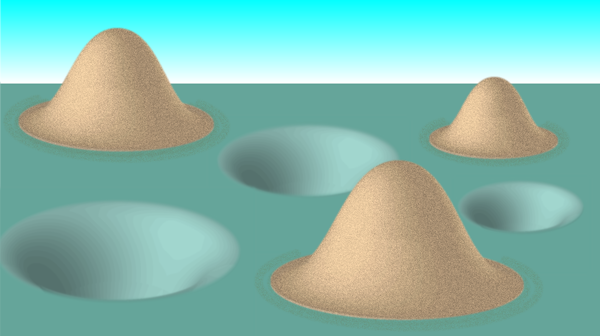
\includegraphics[width=0.5\paperwidth]{figs/piles.png}}
\caption{How do you best move given piles of sand to fill up given holes of the same total volume?}
\label{fig:piles}
\end{figure}

\end{frame}


\begin{frame}{Optimal Mass Transport}{The initial formulation by Monge\cite{monge1781memoire}}
\textbf{Monge Problem}
In the 18th century, Monge first introduced a problem minimizing the inter-domain transportation cost while preserving measure quantities.With modern notations, it can be stated as follows:
\begin{mypro}
Given two probability measures $\mu \in \mathbb{P}(X)$ and $\nu \in \mathbb{P}(Y) $, and a cost function $c : X \times Y \rightarrow [0,+\infty]$, solve $$\inf \{M(T) := \int c(x,T(x)) d\mu(x): T_{\#}\mu=\nu\}$$
where we recall that the measure denoted by $T_{\#}\mu$ is defined through $(T_{\#}\mu)(A):=\mu(T^{-1}(A))$ for every A, and is called image measure or push-forward of $\mu$ through T.
\label{Pro:Monge}
\end{mypro}

\end{frame}

% Page 6
\begin{frame}{Optimal Mass Transport}{The relaxation of Kantorovich for Monge's Problem}
\textbf{Kantorovich Problem} Monge Problem makes it possible to merge mass but not to split mass. To overcome this difficulty, Kantorovich\cite{kantorovich1942transfer} proposed a relaxation of problem where mass can be both splitted and merged .
\begin{mypro}
Given $\mu \in \mathbb{P}(X), \nu \in \mathbb{P}(Y)$ and $c:X\times Y \rightarrow [0,+\infty]$ we consider the problem $$\inf \{K(\gamma):=\int_{X\times Y}cd\gamma: \gamma \in \Pi(\mu, \nu) \}$$
where $\Pi(\mu ,\nu)$ is the set of the so-called transport plans, $$\Pi(\mu,\nu) = \{\gamma \in \mathbb{P}(X\times Y):(\pi_x)_{\#}\gamma = \mu, (\pi_y)_{\#}\gamma = \nu\}$$
where $\pi_x$ and $\pi_y$ are the two projections of $X\times Y$ onto $X$ and $Y$.
\label{Pro:Kanto}
\end{mypro}
\end{frame}


\begin{frame}
Figure[\ref{fig:mapplan}] shows the difference between Transport Map and Transport Plan.
\begin{figure}
\centering
\makebox[\textwidth]{

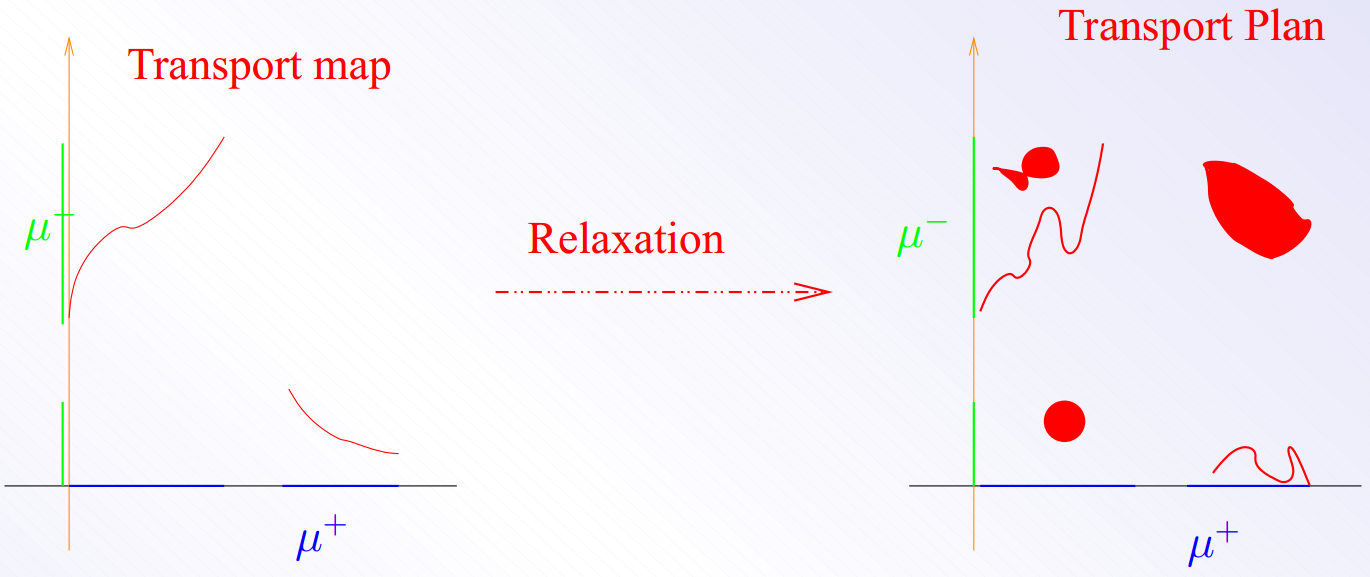
\includegraphics[width= 0.9 \textwidth]{figs/map-vs-plan.png}

}
\caption{Transport Map vs Transport Plan}
\label{fig:mapplan}
\end{figure}

\end{frame}


% Page 7
\begin{frame}{Optimal Mass Transport}

The existence of such transport plans is guaranteed by the following theorems \cite{santambrogio2015optimal}
\begin{theorem}
Let $X$ and $Y$ be compact metric spaces, $\mu\in P(X)$, $\nu\in P(Y)$ and $c:X\times Y\rightarrow\mathbb{R}$ be a continuous function. Then Problem \ref{Pro:Kanto} has a solution.
\label{1.4}
\end{theorem}
\begin{theorem}
Let $X$ and $Y$ be compact metric spaces, $\mu\in P(X)$, $\nu\in P(Y)$ and $c:X\times Y\rightarrow\mathbb{R}\cup \{+\infty\}$ be a lower semi-continuous and bounded from below. Then Problem \ref{Pro:Kanto} has a solution.
\end{theorem}
\end{frame}

%Page 9-1



\subsection{Theory Background}

% page 9
\begin{frame}{Framework of Theory Concepts}
Figure[\ref{fig:pipeline}] shows the whole framework relationship of the theory concepts enrolled in my presentation.
\begin{figure}
\centering
\makebox[\textwidth]{

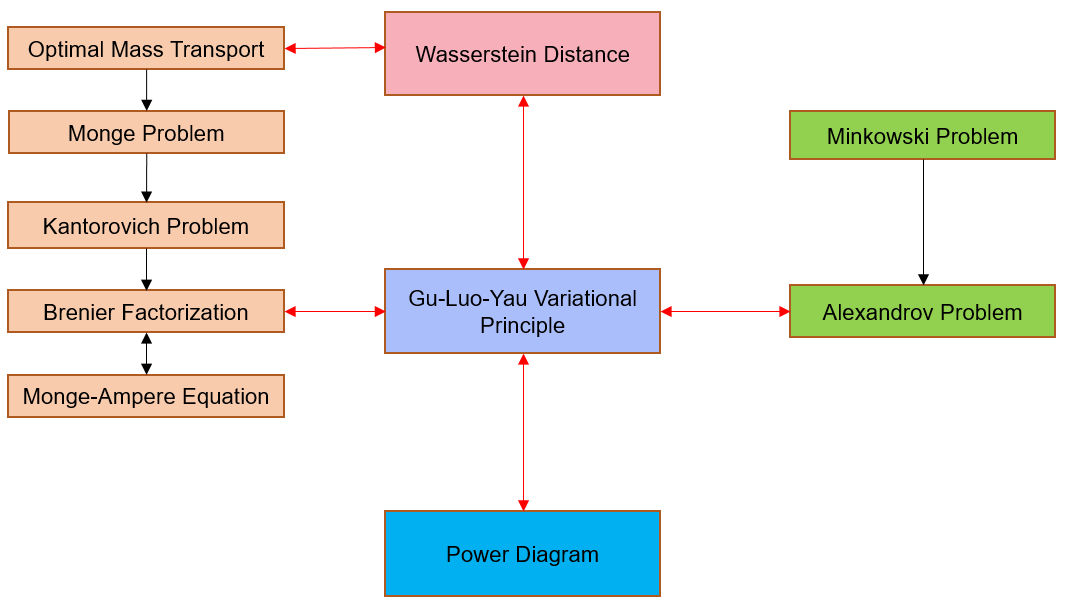
\includegraphics[height= 0.5 \textwidth]{figs/pipeline.png}

}
\caption{The framework of theory concepts}
\label{fig:pipeline}
\end{figure}

\end{frame}

% page 10
\begin{frame}{Convex Geometry}{Minkowski Problem}
\begin{mypro}
(\textbf{Minkowski problem for compact polytopes in $\mathbb{R}^n$}.) Suppose $n_1, n_2, ..., n_k$ are unit vectors which span $\mathbb{R}^n$ and $A_1,..., A_k>0$ so that $\sum^k_{i=1}A_in_i=0$. Find a compact convex polytope $P\subset \mathbb{R}^n$ with exactly k codimension-1 faces $F_1,...,F_k$ so that $n_i$ is the outward normal vector to $F_i$ and the area of $F_i$ is $A_i$.
\end{mypro}
\begin{figure}
\centering
\makebox[\textwidth]{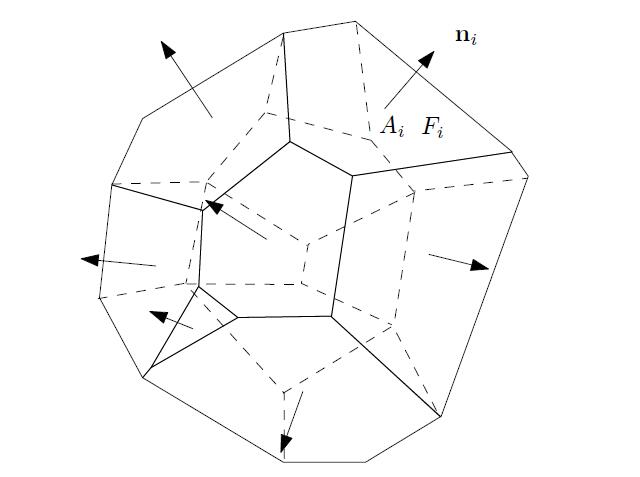
\includegraphics[width=0.3\paperwidth]{figs/MinPro.jpg}}
\caption{Minkowski problem}
\label{fig:Mink}
\end{figure}
\end{frame}

% page 11
\begin{frame}{Convex Geometry}{Alexandrov Theorem}
\begin{theorem}
\textbf{Alexandrov Theorem} Suppose $\Omega$ is a compact convex polytope with non-empty interior in $\mathbb{R}^n$, $p_1, ... , p_k\subset \mathbb{R}^n$ are distinct k points and $A_1,...,A_k>0$ so that $\sum^k_{i=1}A_i=vol(\Omega)$. Then there exists a vector $h =(h_1,...,h_k)\in \mathbb{R}^k$, unique up to adding the constant$(c,c,...,c)$, so that the piecewise linear convex function $$u(x)=\max_{1\leq i\leq k}\{x\cdot p_i + h_i\}$$ satisfies $vol(\{x\in \Omega | \nabla u(x)=p_i\})=A_i$
\end{theorem}
\end{frame}

% page 12
\begin{frame}{Convex Geometry}{Alexandrov Theorem}
\begin{itemize}
\item The graph of the convex function $u$ is an infinite convex polyhedron.
\item The PL convex function produces a convex cell decomposition $\{W_i\}$
\end{itemize}
\begin{figure}
\centering
\makebox[\textwidth]{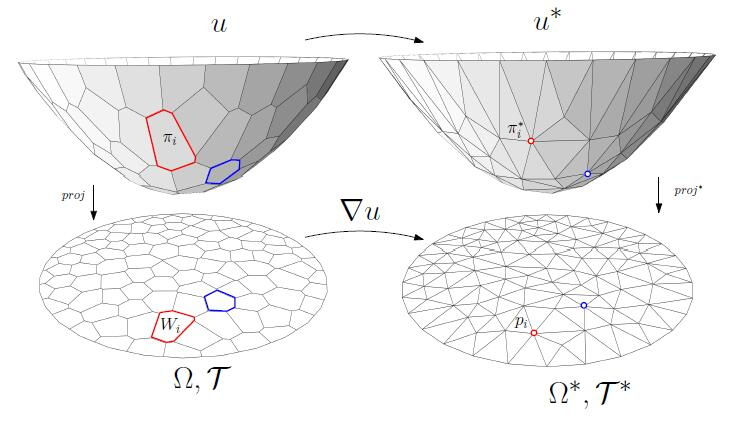
\includegraphics[width=0.6\paperwidth]{figs/AlePro.jpg}}
\caption{A PL convex function induces a cell decomposition of $\Omega$. Each cell maps to a point}
\label{fig:Alex}
\end{figure}
\end{frame}



\begin{frame}{Brenier's Polar Factorization}
\begin{theorem}
(Polar Factorization\cite{brenier1991polar}). Let $\Omega_0$ and $\Omega_1$ be two convex subdomains of $\mathbb{R}^n$ with smooth boundaries, each with a positive density function $\mu_0,\mu_1$ respectively, and of the same total mass $\int_{\Omega_0}\mu_0=\int_{\Omega_1}\mu_1$. Let $\phi:(\Omega_0,\mu_0)\rightarrow (\Omega_1, \mu_1)$ be an diffeomorphic mapping, then $\phi$ has a unique decomposition of the form $$\phi=(\nabla u)\circ s$$ where $u:\Omega_0\rightarrow \mathbb{R}$ is a convex function, $s:(\Omega_0,\mu_0)\rightarrow(\Omega_0,\mu_0)$ is a measure-preserving mapping. This is called a polar factorization of $\phi$ with respect to $\mu_0$.
\label{Thm:polarfac}
\end{theorem}
\end{frame}

\begin{frame}{Brenier's Polar Factorization}
A diffeomorphism $\phi:(\Omega_0,\mu_0)\rightarrow (\Omega_1, \mu_1)$, where $\mu_1=\phi_\#\mu_0$, can be decomposed to the composition of a measure preserving map $s:(\Omega_0,\mu_0)\rightarrow (\Omega_0, \mu_0)$ and a $L^2$ optimal mass transport map~\cite{brenier1991polar} $\nabla u:(\Omega_0,\mu_0)\rightarrow (\Omega_1, \mu_1)$, and the composition is unique.\\

According to \textit{Polar Decomposition}, $\nabla u^*=(\nabla u)^{-1}:(\Omega_1, \mu_1)\rightarrow (\Omega_0,\mu_0)$ is also an optimal mass transportation map. The measure-preserving map $s$ can be computed directly by $s=(\nabla u)^{-1}\circ \phi$.
\end{frame}



% page 13
\begin{frame}{Convex Geometry}{Alexandrov Theorem}
\begin{mydef}
\textbf{Alexandrov map} The gradient map $\nabla u:x\mapsto\nabla u(x)$ is the Alexandrov map.
\label{def:alexmap}
\end{mydef}
\begin{itemize}
\item $u$ and $\nabla u(x)$ in the theorem is called the $Alexandrov$ $ potential$ and $Alexandrov$ $map$
\item $Alexandrov$ $ map$ is the unique OMT map
\item The gradient map minimizes the energy $$\int _\Omega||x-T(x)||^2dx$$
\end{itemize}
\end{frame}

% page 14
\begin{frame}{Variational Principle}
\begin{theorem}
Let $\Omega$ be a compact convex domain in $\mathbb{R}^n$ and $\{p_1,...,p_k\}$ a set of distinct points in $\mathbb{R}^n$ and $\sigma:\Omega \rightarrow \mathbb{R}$ be a positive continuous function. Then for any $A_1,...,A_k>0$ with $\sum^k_{i=1}A_i=\int_\Omega \sigma(x)dx$, there exists $b=(b_1,...,b_k)\in \mathbb{R}^k$, unique up to adding a constant $(c,...,c)$, so that $\int_{W_i(b)\cap\Omega}\sigma(x)dx=A_i$ for all $i$. The vectors b are exactly minimum points of the convex function $$E(h) = \int ^h_a \sum^k_{i=1}\int_{W_i(h)\cap \Omega}\sigma(x)dxdh_i-\sum^k_{i=1}h_iA_i$$
on the open convex set $H=\{h\in\mathbb{R}^k|vol({W_i(h)\cap \Omega})>0  \forall i\}$.
\label{thm:1.2}
\end{theorem}
\end{frame}

% page 15
\begin{frame}{Variational Principle}
\begin{block}{Theorem \ref{thm:1.2}}
(continued) In fact, $E(h)$ restricted to $H_0=H\cap\{h|\sum^k_{i=1}h_i=0\}$ is strictly convex. Furthermore, $\nabla u_b$ minimizes the quadratic cost $\int_{\Omega}|x-T(x)|^2\sigma dx$ among all transport maps $T:(\Omega, \sigma dx)\rightarrow(\mathbb{R}^n,\sum^k_{i=1}A_i\delta_{p_i})$. where $u_b$ is defined as the PL convex function $$u_b(x)=\max_i\{x\cdot p_i+b_i\}$$
and the closed convex polytope is denoted as $$W_i(h)=\{x\in \mathbb{R}^n|\nabla u(x)=p_i\}=\{x|x\cdot p_i+b_i\geq x\cdot p_j+b_j\ for\ all\ j\}$$
\end{block}
\end{frame}

% page 16
\begin{frame}{Computational Geometry}{Power Diagram}
\begin{itemize}
\item Voronoi Diagram
$\forall\ p$, the convex region $R(p)=\{x\in E^d | d(x,p) \leq d(x,q), \forall q \in M-\{p\}\}.$
\item Power Voronoi Diagram use the power distance. $$POW(x,p_i)=\dfrac{1}{2}||x-p_i||^2-\dfrac{1}{2}h_i.$$
\item Power Diagram is a partition of Euclidean plane,
$$W_i=\{x|Pow(x,p_i)\leq Pow(x,p_j), \forall j\}.$$
\item Computing the Power Diagram is equivalent to computing the Alexandrov map.
\end{itemize}
\end{frame}

% page 17
\begin{frame}{Computational Geometry}{Power Diagram}
\begin{figure}
\centering
\makebox[\textwidth]{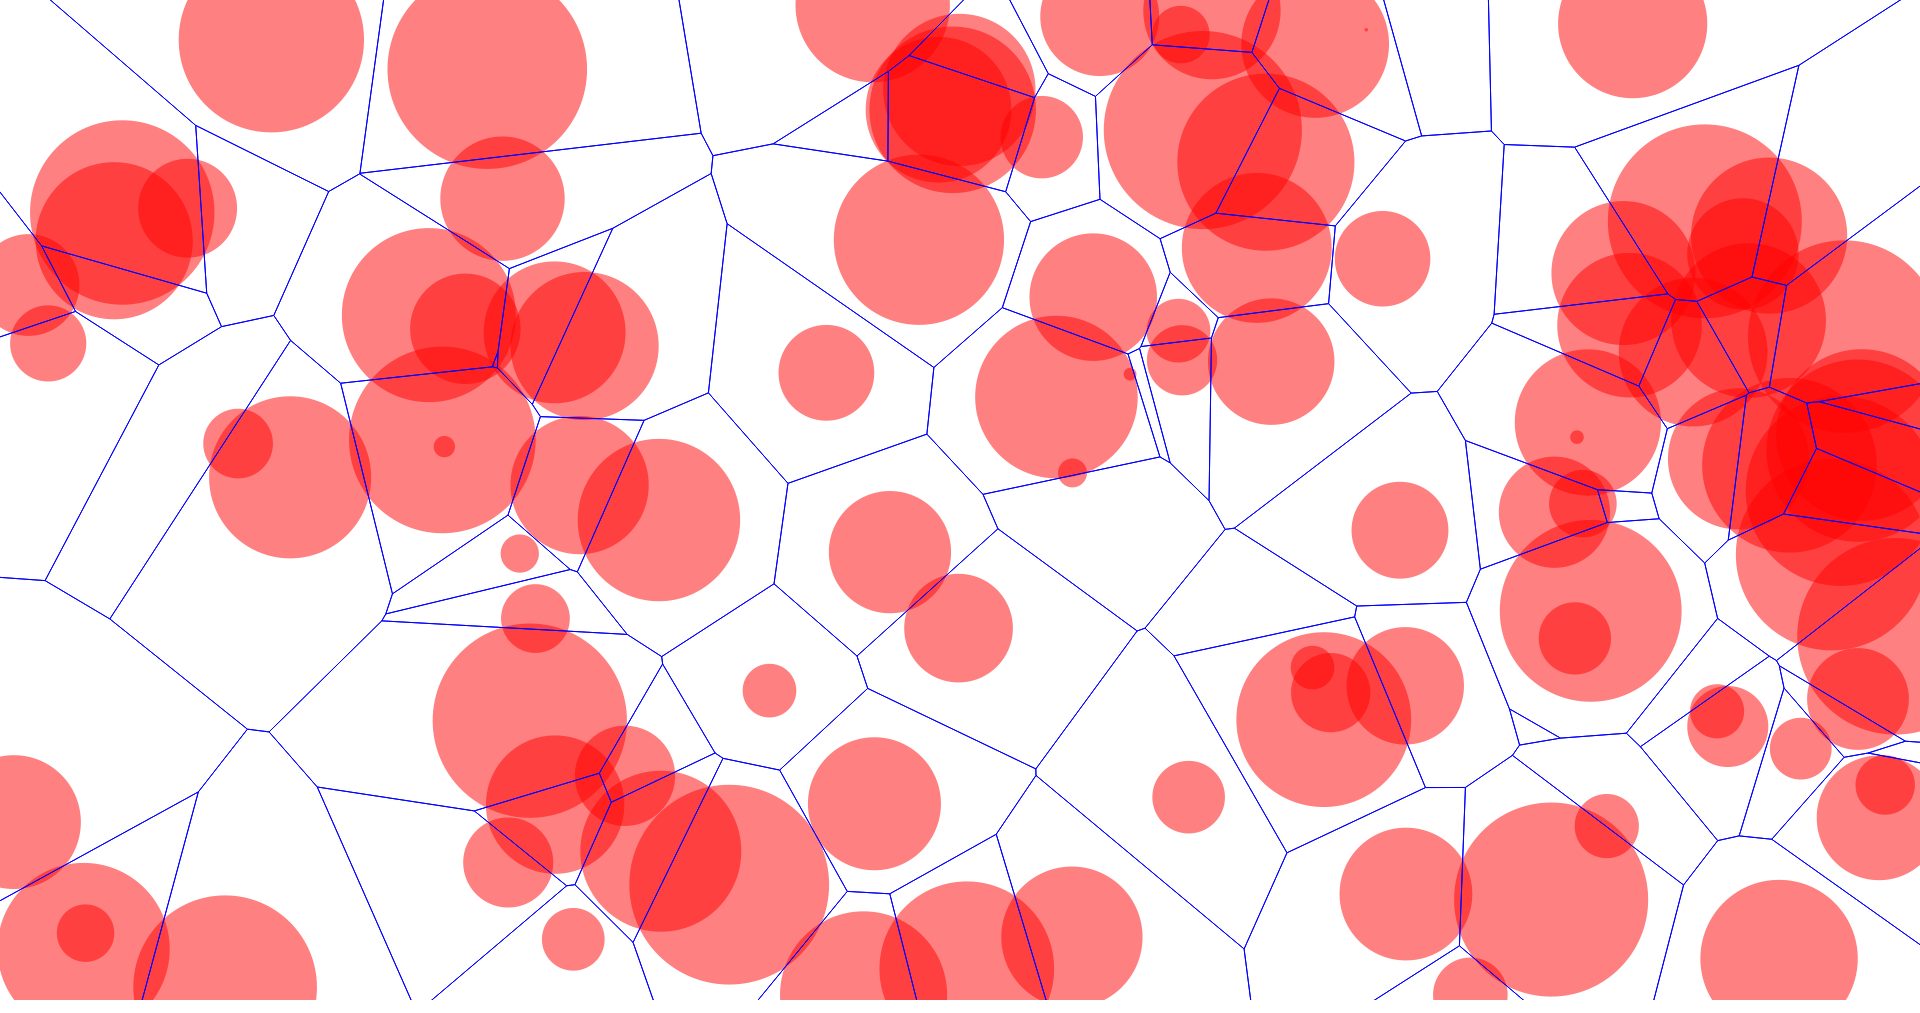
\includegraphics[width=0.6\paperwidth]{figs/full.png}}
\caption{Power diagram.}
\label{fig:PowDia}
\end{figure}

\end{frame}

% page 18
\begin{frame}{Monge-Ampere Equation\cite{de2014monge}}

\begin{theorem}
Let $\mu$ and $\nu$ be two compactly supported probability measure on $\mathbb{R}^n$. If $\mu$ is absolutely continuous with respect to the Lebesgue measure, then
\begin{itemize}
\item[i.] there exists a unique solution $T$ to the optimal mass transport problem with cost $c(x,y)=|x-y|^2/2$;
\item[ii.] there exists a convex function $u:\mathbb{R}^n\rightarrow\mathbb{R}$ such that the optimal map $T$ is given by $T(x)=\nabla u(x)$ for $\mu-a.e.\ x$
\end{itemize}

\label{thm:OMT_MAE}
\end{theorem}
\end{frame}

% page 19
\begin{frame}{Monge-Ampere Equation}
\begin{block}{Theorem \ref{thm:OMT_MAE}}
(continued) Furthermore, if $\mu(dx)=f(x)dx$ and $\nu(dy)=g(y)dy$, then $T$ is differentiable $\mu-a.e.$ and $$|det(\nabla T(X))|=\dfrac{f(x)}{g(T(x))}\ \ \ for\ \mu-a.e.\ x\in\mathbb{R}^n.$$
\end{block}
Since $T=\nabla u$,\cite{brenier1991polar}, the formula becomes:
$$det(D^2u(x))=\dfrac{f(x)}{g(\nabla (u))}$$ which is a non-linear elliptic PDE.
\end{frame}

% page 20
\begin{frame}{Wasserstein Distance}
\begin{mydef}
\textbf{Shape Distance} Given two Riemannian surfaces, which are topological disks, $(S_1,\mathbf{g}_1)$ and $(S_2,\mathbf{g}_2)$, the Riemann mappings are $\phi_k$, $k=1,2$ respectively. Let $\eta\in  Mob(\mathbb{D})$ be a Mobius transformation, where $Mob(\mathbb{D})$ is the Mobius transformation group of the unit planar disk, then $\eta_k\circ \phi_k$ is still Riemann mapping. Each Riemann mapping $\eta_k\circ \phi_k$ determines a unique optimal mass transportation map $\tau_k(\phi_k,\eta_k)$. Then the distance between two surfaces is given by $$d(S_1,S_2) := \min_{\eta_1,\eta_2\in Mob(\mathbb{D})}\int_\mathbb{D}|\tau_1(\phi_1,\eta_1)-\tau_2(\phi_2,\eta_2)|^2dxdy$$
\end{mydef}
\end{frame}

%page 21
\begin{frame}{Wasserstein Distance}
\textbf{Wasserstein Metric Space}$(M, \mathbf{g})$ is a Riemannian manifold with a Riemannian metric $\mathbf{g}$, considering the set: $$P_p(M):=\{\mu\in P(M): \int|x|^pd\mu<+\infty\}.$$
For $\mu,\nu\in P_p(M)$, we define $$W_p(\mu,\nu):=\inf_{T_\#\mu=\nu}(\int_Md(x,T(x))^pd\mu(x))^{\frac{1}{p}}.$$
\begin{itemize}
\item $W_p(\mu,\nu)\geq 0$.
\item $W_p(\mu,\nu)=0$ implies $\mu = \nu$.
\item Satisfies the triangle inequality.
\end{itemize}
The quantity $W_p$ is the $Wasserstein$ $Distance$ over $P_p(M)$.
\end{frame}


\section{Computational Algorithms In Discrete Settings}

\subsection{Discrete Conformal Mapping}
% page 25
\begin{frame}{Algorithms}{Discrete Conformal Mapping}
\begin{mydef}
(Discrete Metric). A discrete metric on a triangular mesh $(S,T)$ is a function defined on the edges $d:E\rightarrow \mathbb{R}^+$, which satisfies the triangle inequality, on a face $[v_i,v_j,v_k]$, $$d_{ij}+d_{jk}>d_{ki};d_{ki}+d_{ij}>d_{jk};d_{ik}+d_{kj}>d_{ji}.$$
\end{mydef}
\begin{mydef}
(Delaunay Triangulation). A triangulation such that no point is inside the circumcircle of any triangle.
%Aclosed discrete surface $(S,T)$ with a discrete metric $d$, we say a triangulation $T$ is Delaunay, if for any edge $[v_i,v_j]$ adjacent to two faces $[v_i,v_j,v_k]$ and $[v_j,v_i,v_l]$, $$\theta_k^{ij}+\theta_l^{ji}\leq \pi,$$ where $\theta_k^{ij}$ is the corner angle at $v_k$ in $[v_i,v_j,v_k]$, and $\theta_l^{ji}$ is the angle at $v_l$ in $[v_j,v_i,v_l]$.
\end{mydef}
\end{frame}

% page 26
\begin{frame}{Algorithms}{Discrete Conformal Mapping}
\begin{mydef}
(Discrete Gauss Curvature). The discrete Gauss curvature function on a mesh is defined on vertices, $K: V\rightarrow \mathbb{R}$, such that
\[
	K(v)=\begin{cases}
			2\pi-\sum_i\theta_i,\ v\notin\partial S\\
			\pi-\sum_i\theta_i, \ v\in\partial S
		\end{cases}			
\]
where $\theta_i$'s are corner angles adjacent to the vertex $v$, and $\partial S$ represents the boundary of the mesh.

Gauss-Bonnet:
$$\sum_i K(v_i)=2\pi\chi(S)$$
where $\chi(S)$ is the Euler characteristic of $S$.
\end{mydef}
\end{frame}

% page 27
\begin{frame}{Algorithms}{Discrete Yamabe Flow}
\begin{mydef}
(Discrete Yamabe Flow). Given a surface $(S,V)$ with a discrete metric $d$, given a target curvature function $\bar{K}:V\rightarrow \mathbb{R},\ \bar{K}(v_i)\in(-\infty,2\pi)$, and the total target curvature satisfies Gauss-Bonnet formula, the discrete Yamabe flow is defined as $$\dfrac{du(v_i)}{dt}=\bar{K}(v_i)-K(v_i),$$
under the constraint $\sum_{v_i\in V}u(v_i) = 0$. As the Yamabe flow updates at each iteration, the triangulation on $(S,V)$ always keep the property of the Delaunay triangulation.


\end{mydef}
The existence of the solution to the Yamabe flow is guarranteed by the following theorem.
\end{frame}

\begin{frame}{Algorithms}{Discrete Yamabe Flow}
\begin{theorem}
Suppose $(S,V)$ is a closed connected surface and $d$ is any discrete metric on $(S,V)$. Then for any $\bar{K}:V\rightarrow (-\infty,2\pi)$ satisfying Gauss-Bonnet formula, there exists a discrete metric $\bar{d}$, unique up to a scaling on $(S,V)$, so that $\bar{d}$ is discrete conformal to $d$ and the discrete curvature of $\bar{d}$ is $\bar{K}$. Furthermore, the $\bar{d}$ can be obtained by discrete Yamabe flow.
\end{theorem}
\end{frame}

% Page 29
\begin{frame}{Algorithms}
\begin{algorithm}[H]

\begin{algorithmic}[1]
	\REQUIRE: A triangular mesh $\Sigma$, A target curvature $\bar{K}$

	\ENSURE: A discrete metric
  	\STATE Initialize the discrete conformal factor $u$ as 0 and conformal structure coefficient $\eta$, such that $\eta(e)$ equals to the initial edge length of $e$.
  	\WHILE{$\max_i|\bar{K}_i-K_i|>\epsilon$}
  	\STATE compute the edge length from $\gamma$ and $\eta$
  	\STATE (Update the triangulation to be Delaunay using diagonal edge swap for each pair of adjacent faces)
  	\STATE Compute the corner angle $\theta^{jk}_i$ from the edge length using cosine law
  	\STATE Compute the vertex curvature $K$
  	\STATE Compute the Hessian matrix $H$
  	\STATE Solve linear system $H\delta u=\bar{K}-K$
  	\STATE Update conformal factor $u\leftarrow u-\delta u$
  	\ENDWHILE
  	\STATE Output the result metric
\end{algorithmic}
\caption{Discrete Surface Yamabe Flow}
\end{algorithm}
\end{frame}

\begin{frame}{Algorithms}{Discrete Yamabe Flow}
The Hessian matrix $H$ is defined explicitly:
\[
	h_{ij} = \begin{cases}
			-w_{ij} & v_i\sim v_j\  i\neq j \\
			0  &v_i\nsim v_j \ i\neq j \\
			\sum_k w_{ik}  &i=j
		\end{cases}
\]
where $w_{ij}$ is the cotangent edge weight defined as
\[
w_{ij} := \begin{cases}
		cot\theta^{ij}_k+cot\theta^{ji}_l &[v_i,v_j]\notin \partial S \\
		cot\theta^{ij}_k &[v_i,v_j]\in \partial S
	\end{cases}
\]
\end{frame}


% Page 41
\subsection{Brenier's Polar Factorization}

% Page 43
\begin{frame}{Algorithm}{Polar Factorization}
\begin{algorithm}[H]
\caption{Polar Factorization of Mapping}
\begin{algorithmic}
\REQUIRE Convex domains $\Omega_0$ and $\Omega_1$ in $\mathbb{R}^d$. A diffeomorphic mapping $\phi:(\Omega_0,\mu_0)\rightarrow (\Omega_1, \mu_1)$, satisfying $\mu_1=\phi_\#\mu_0$.
\ENSURE The polar factorization $\phi = \nabla u\circ s$, where $s$ is measure-preserving and $u$ is convex.
\STATE Compute the unique optimal mass transport map $\nabla v:(\Omega_1, \mu_1)\rightarrow (\Omega_0,\mu_0)$ using Alg.\ref{algo:DOMT}. The convex function $u$ is the Legendre dual of $v$, $u=v^*$
\STATE Compute the composition $s=\nabla v\circ\phi$
\end{algorithmic}
\label{Algo:PolarFac}
\end{algorithm}
\end{frame}


\subsection{Discrete Optimal Mass Transport}
%\begin{frame}{Algorithms}{Discrete Optimal Mass Transport}
%\begin{theorem}
%For any given measure $\nu$, such that $$\sum^n_{j=1}\nu_j=\int_\Omega \mu, \nu_j>0,$$ there must exist a height vector $\mathbf{h}$ unique up to adding a constant vector $(c,c,...,c)$, the convex function $u_\mathbf{h}(x)$ induces the cell decomposition of $\Omega = \cup^k_{i=1}W_i(\mathbf{h})$, such that the following area-preserving constraints are satisfied for all cells, $$\int_{W_i(\mathbf{h})}\mu(x)=\nu_i,\ i=1,2,...,n. $$
%\label{thm:5}
%\end{theorem}
%\end{frame}
%
%\begin{frame}{Algorithms}{Discrete Optimal Mass Transport}
%\begin{block}{Theorem \ref{thm:5}}
%Furthermore, the gradient map $grad\ u_{\mathbf{h}}$ optimizes the transportation cost $$C(T):=\sum_\Omega|x-T(x)|^2\mu(x)dx.$$
%\end{block}
%\end{frame}

\begin{frame}{Algorithms}{Discrete Optimal Mass Transport}
\begin{theorem}
Let $\Omega$ be a compact convex domain in $\mathbb{R}^n$, $\{p_1,...,p_k\}$ be a set of distinct points in $\mathbb{R}^n$ and $\sigma:\Omega\rightarrow \mathbb{R}$ be a positive continuous function. Then for any $A_1,...,A_k>0$ with $\sum^k_{i=1}A_i=\int_{\Omega}\sigma(x)dx,$ there exists $b=(h_1,...,h_k)\in \mathbb{R}^k$, unique up to adding a constant $(c,c,...,c)$, so that $\int_{W_i(b)\cap \Omega}\sigma(x)dx=A_i$ for all $i$. The vectors $b$ are exactly minimum points of the convex function $$E(h)=\int^h_a\sum^k_{i=1}\int_{W_i(h)\cap\Omega}\sigma(x)dxdh_i-\sum^k_{i=1}h_iA_i$$ on the open convex set $H=\{h\in\mathbb{R}^k|vol(W(h)\cap \Omega)>0\ for\ all\ i\}$. Furthermore, $\nabla u_h$ minimizes the quadratic cost $\int_\Omega|x-T(x)|^2\sigma(x)dx$ among all transport maps $T:(\Omega,\sigma dx)\rightarrow(\mathbb{R}^n,\sum^k_{i=1}A_i\delta_{p_i})$
\end{theorem}
\end{frame}

\begin{frame}{Algorithms}{Discrete Optimal Mass Transport}
In practice, the energy can be optimized using Newton's method, with the help of the computation of the energy gradient $$\nabla E(\mathbf{h})=(w_1(\mathbf{h})-\nu_1,...,w_k(\mathbf{h})-\nu_k)^T$$. The Hessian of $E(\mathbf{h})$ is given as following:
\[
\dfrac{\partial ^2E(\mathbf{h})}{\partial h_i\partial h_j}=\begin{cases}
					\frac{\int_{e_{ij}}\mu(x)dx}{|y_j-y_i|}\ &W_i(\mathbf{h})\cap W_j(\mathbf{h})\cap \Omega\neq\emptyset \\
					0 &otherwise
\end{cases}
\]
\end{frame}

% Page 35
\begin{frame}
\begin{algorithm}[H]
\begin{algorithmic}[1]
	\REQUIRE \textbf{The Input:} $(\Omega,\mu)$,$(P,\nu),\nu_i>0,\int_\Omega u(x)dx=\sum^k_{i=1}\nu_i$ \\
%	\begin{enumerate}
%	\item[1.] A convex planar domain with measure $(\Omega,\mu)$;
%	\item[2.] A planar point set with measure $(P,\nu),\nu_i>0,\int_\Omega u(x)dx=\sum^k_{i=1}\nu_i$
%	\end{enumerate}
	\textbf{The Output:} The unique discrete OMT-Map $f:(\Omega,\mu)\rightarrow(P,\nu)$
	
  	\STATE Scale and translate P, such that $P\subset \Omega$
  	\STATE $\mathbf{h}\leftarrow(0,0,...,0)$
  	\STATE Compute the power diagram $D(\mathbf{h})$,dual power Delaunay triangulation $T(\mathbf{h})$,the cell areas $\mathbf{w}(\mathbf{h})=(w_1(\mathbf{h}),...,w_k(\mathbf{h}))$
  	\WHILE{$||\nabla E||<\epsilon$}
  	\STATE Compute $\nabla E$ and Hessian matrix
  	\STATE $\lambda\leftarrow 1$
  	\STATE $\mathbf{h}\leftarrow \mathbf{h}-\lambda H^{-1}\nabla E(\mathbf{h})$
  	\STATE Compute $D(\mathbf{h})$, $T(\mathbf{h})$, and $\mathbf{w}(\mathbf{h})$
  		\WHILE{$\exists w_i(\mathbf{h})==0$}
  		\STATE Update $\mathbf{h}\leftarrow \mathbf{h}+\lambda H^{-1}\nabla E(\mathbf{h})$, $\lambda\leftarrow\frac{1}{2}\lambda$,$\mathbf{h}\leftarrow \mathbf{h}-\lambda H^{-1}\nabla E(\mathbf{h})$
%  		\STATE $\lambda\leftarrow\frac{1}{2}\lambda$
%  		\STATE $\mathbf{h}\leftarrow \mathbf{h}-\lambda H^{-1}\nabla E(\mathbf{h})$
  		\STATE Compute $D(\mathbf{h})$, $T(\mathbf{h})$, and $\mathbf{w}(\mathbf{h})$
  		\ENDWHILE
  	\ENDWHILE
  	\STATE Output the result mapping $f:\Omega\rightarrow P, W_i(\mathbf{h})\rightarrow p_i,\ i=1,2,...,k.$
\end{algorithmic}
\caption{Optimal Mass Transport Map}
\label{algo:DOMT}
\end{algorithm}
\end{frame}

% Page 36
\subsection{Area-preserving Map For Topological Disks}
\begin{frame}{Algorithms}{Area-preserving map for topological disks}
Suppose $S$ is a topological disk, with Riemannian metric $g$. Scale the surface so that the area is $\pi$. According to Riemann Mapping theorem, there is a conformal mapping $\phi :(S,\mathbf{g})\rightarrow(\mathbb{D},dzd\bar{z})$, such that $\mathbf{g}= e^{2\lambda(z)}dzd\bar{z}$. Then we can find the OMT map $\tau:(\mathbb{D},dzd\bar{z})\rightarrow (\mathbb{D},e^{2\lambda}dzd\bar{z})$, and the composition $\tau^{-1}\circ \phi:(S,\mathbf{g})\rightarrow(\mathbb{D},dzd\bar{z})$ gives the area-preserving mapping.
\end{frame}

% Page 40
\begin{frame}{Algorithms}{Area-preserving map for topological disks}
\begin{algorithm}[H]
\caption{Topological Disk Area-preserving Parameterization}
\begin{algorithmic}[1]
	\REQUIRE \textbf{The inputs:} a triangular mesh $M$, which is a topological disk; three vertices $\{v_0,v_1,v_2\}\subset \partial M$ \\
	\textbf{The output:} The area-preserving parameterization $f:M\rightarrow \mathbb{D}$, which maps $\{v_0,v_1,v_2\}$ to $\{1,i,-1\}$ respectively.
	\STATE Scale $M$ such that the total area is $\pi$
	\STATE Compute the conformal parameterization $\phi:M\rightarrow\mathbb{D}$, such that the images of $\{v_0,v_1,v_2\}$ are $\{1,i,-1\}$
	\STATE For each vertex $v_i\in M$, define $p_i=\phi(v_i)$, $\nu_i$ to be $\frac{1}{3}$ of the total area of the faces adjacent to $v_i$. Set $P=\{p_i\},\nu=\{\nu_i\}$
	\STATE Compute the \textit{Discrete Optimal Mass Transport Map} with Algorithm \ref{algo:DOMT}
	\STATE Construct the mapping $\tau^{-1}\circ\phi:M\rightarrow\mathbb{D}$, which maps each vertex $v_i\in M$ to the centroid of $W_i(\mathbf{h})\subset \mathbb{D}$
\end{algorithmic}
\end{algorithm}
\end{frame}

% Page 46
\subsection{Discrete Conformal Wasserstein Distance}
\begin{frame}{Algorithm}{Discrete Conformal Wasserstein Distance}
After we have the OMT map between two surfaces $M_1$, $M_2$ with topological disk algorithm, we will have the map: $f:\Omega\rightarrow P, W_i(\mathbf{h})\rightarrow p_i$. Therefore, the Wasserstein distance between $M_1$ and $M_2$ can be defined as $$d_W(\mu,\nu)=\sum^n_{i=1}\int_{W_i}(x-p_i)^2\mu(x)dx$$
\end{frame}
% Page 47
\begin{frame}{Algorithm}{Conformal Wasserstein Distance}
\begin{algorithm}[H]
\caption{Computing Wasserstein Distance for Two Surfaces}
\begin{algorithmic}[1]
\REQUIRE \textbf{Input:} Two topological disk surfaces: $(M_1,g_1), (M_2,g_2)$. \\
\textbf{Output:} The Wasserstein distance between $M_1$ and $M_2$
\STATE Scale and normalize $M_1$ and $M_2$ such that the total area of each is $\pi$.
\STATE Compute the conformal maps $\phi_1:M_1\rightarrow \mathbb{D}_1$, and $\phi_2:M_2\rightarrow \mathbb{D}_2$ defined above.
\STATE Construct the convex planar domain $(\Omega,\mu)$ from $\mathbb{D}_1$, $\mu \leftarrow e^{2\lambda_1}d_A$
\STATE Discretize $\mathbb{D}_2$ into a planar point set with measure $(P,\nu)$
\STATE With $(\Omega, \mu)$ and $(P,\nu)$ as inputs, compute the Optimal Mass Transport map $f$ with Algorithm \ref{algo:DOMT}
\STATE Output the Wasserstein distance $d_W(\mu,\nu)$.
\end{algorithmic}
\label{Algo:WasDis}
\end{algorithm}
\end{frame}

\section{Applications}
\subsection{Wasserstein Distance for Shape Analysis}

%Page 48
\begin{frame}{Wasserstein Distance for Shape Analysis}{Hippocampal Surface Classification}
Utilizing the Wasserstein distance to classify the patients' and normal person's hippocampus.  
Table[\ref{fig:textures}] and Fig.[\ref{fig:ROC1}] demonstrate our method has better classification performance than other methods.
\end{frame}

%Page 49
\begin{frame}{Wasserstein Distance for Shape Analysis\cite{su2015optimal}}{Surface Matching}
\begin{figure}
\centering
\makebox[\textwidth]{\begin{tabular}{cccc}
\epsfig{file=./figs/normal_left_checkerboard.eps,width=0.15 \textwidth}&
\epsfig{file=./figs/normal_right_checkerboard.eps,width=0.15 \textwidth}&
\epsfig{file=./figs/epilepsy_left_checkerboard.eps,width=0.15 \textwidth}&
\epsfig{file=./figs/epilepsy_right_checkerboard.eps,width=0.15 \textwidth}\\
(a) & (b) & (c) & (d)\\
\epsfig{file=./figs/normal_left_circle.eps,width=0.15 \textwidth}&
\epsfig{file=./figs/normal_right_circle.eps,width=0.15 \textwidth}&
\epsfig{file=./figs/epilepsy_left_circle.eps,width=0.15 \textwidth}&
\epsfig{file=./figs/epilepsy_right_circle.eps,width=0.15 \textwidth}\\
(e) & (f) & (g) & (h)\\
\end{tabular}}
\caption{Conformal texture-mapping results. (a)-(d) conformal checkerboard-texture mapping results of left and right hippocampus
surfaces in normal control and epilepsy data groups, respectively; (e)-(h)conformal circle-texture mapping results of left and right hippocampus
surfaces in normal control and epilepsy data groups, respectively.}
\label{fig:textures}
\end{figure}
\end{frame}


%Page 50
\begin{frame}

\begin{figure}
\centering
\begin{minipage}[!t]{0.6\textwidth}
\centering
	\includegraphics[width=\textwidth]{figs/ROC1.eps}
	\caption{Comparison of average ROC curves for three methods.}\vspace{3em}
	\label{fig:ROC1}
\end{minipage}%
\end{figure}


\end{frame}





%Page 52
\begin{frame}


\begin{table}
\centering
\caption{Average AUC value.}
\label{tbl:ROC}
\begin{tabular}[\textwidth]{@{\extracolsep{\fill}}lc}
\hline
Methods & Average AUC value\\
\hline
Area Distortion& 0.6948 \\
Curvature Difference & 0.7342\\
Curvature Difference + Area Distortion & 0.7542\\
Wasserstein Distance & 0.8834\\
\hline
\end{tabular}
\end{table}




\end{frame}


%Page 53
\subsection{Optimal Mass Transport For Visualization}
\begin{frame}{Optimal Mass Transport For Visualization}
Our work\cite{su2016area} allows users to fully control the texture area of region of interests, which will be helpful in medical image field. By adjusting the target measure, the user can zoom or shrink specific regions on the surface as shown in Fig.[\ref{fig:roi_face}] and [\ref{fig:roi_skull}]. The top row demonstrates that the user can control the areas of the holes, the bottom row shows the user can enlarge/shrink the nose region with different scaling factors in Fig.[\ref{fig:roi_face}]. The similar observation is also obtained from skull model shown in Fig.[\ref{fig:roi_skull}].
\end{frame}



%Page 53

\begin{frame}{Optimal Mass Transport For Visualization}
\begin{figure}
\centering
\makebox[\textwidth]{
	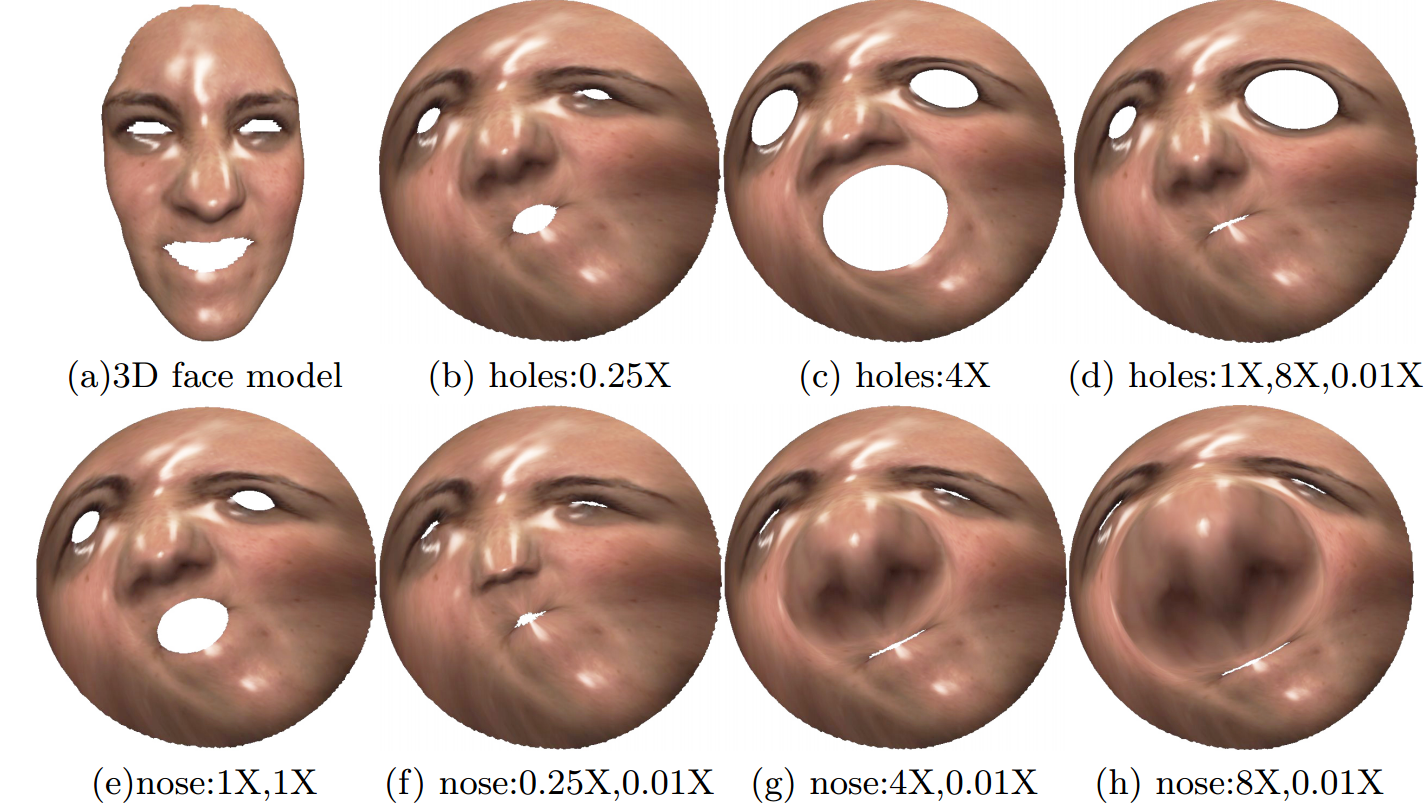
\includegraphics[width= 0.8 \textwidth]{figs/nose.png}

}

\caption{Importance driven surface parameterization for human face; (a) the 3d face model; (b)-(d) shows importance driven results of the holes with different scale factors; (e)-(h) shows the importance driven results of the nose and holes with different scale factors.}
\label{fig:roi_face}
\end{figure}
\end{frame}




\begin{frame}{Optimal Mass Transport For Visualization}
\begin{figure}
\centering
\makebox[\textwidth]{

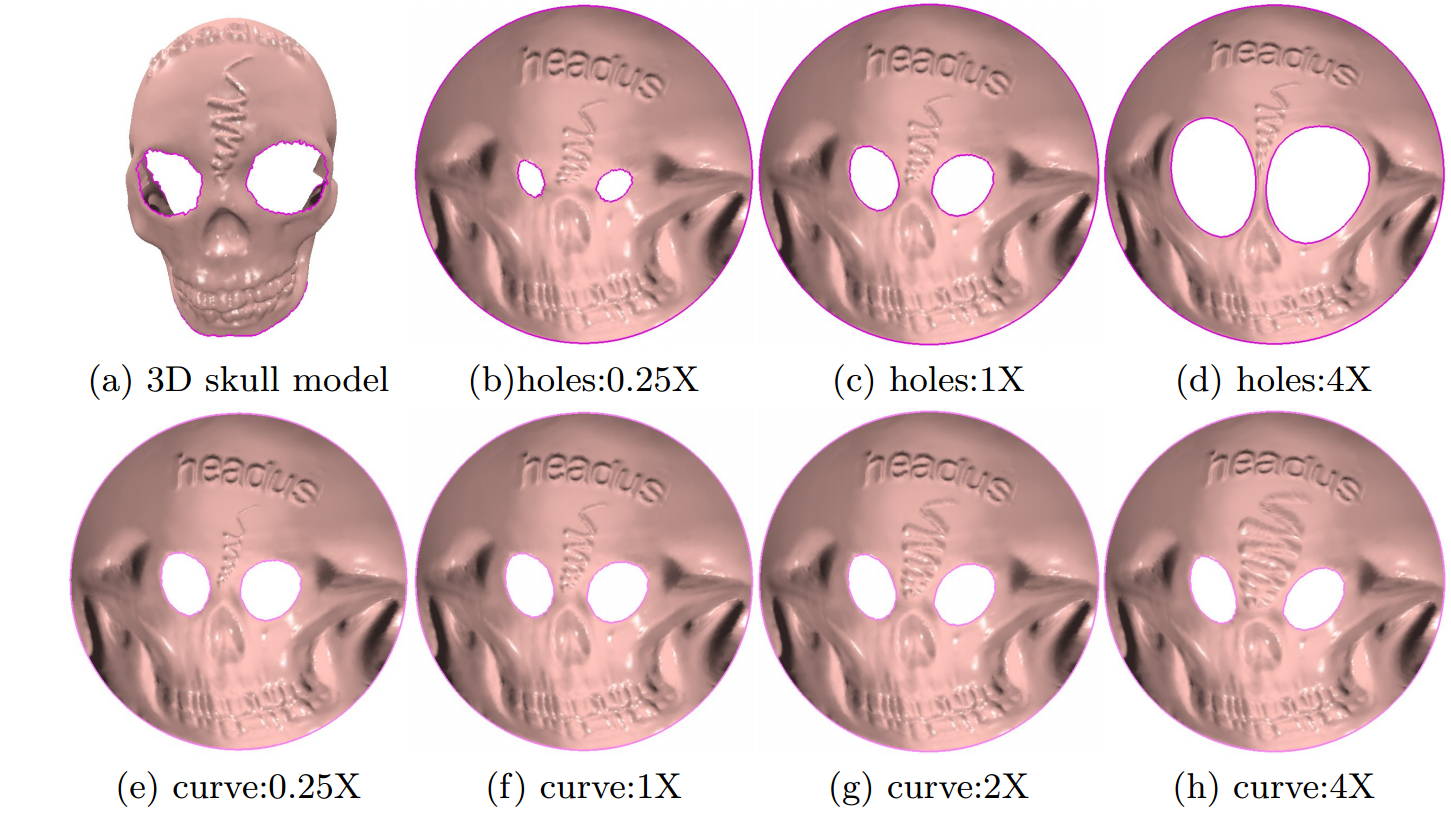
\includegraphics[width= 0.8 \textwidth]{figs/skull.png}

}
\caption{Importance driven surface parameterization for skull; (a) the 3d skull model; (b)-(d) shows importance driven results of the holes with different scale factors; (e)-(h) shows the importance driven results of the curve with different scale factors.}
\label{fig:roi_skull}
\end{figure}
\end{frame}



\subsection{Volume Preserving Morphing}


\begin{frame}{Volume Preserving Morphing}

In our paper\cite{su2016volume}, our OMT method Fig.[\ref{fig:gu_morph}] can produce more smooth morphing result than Fig.[\ref{fig:bruno_morph}].

\begin{figure}
\centering
\makebox[\textwidth]{

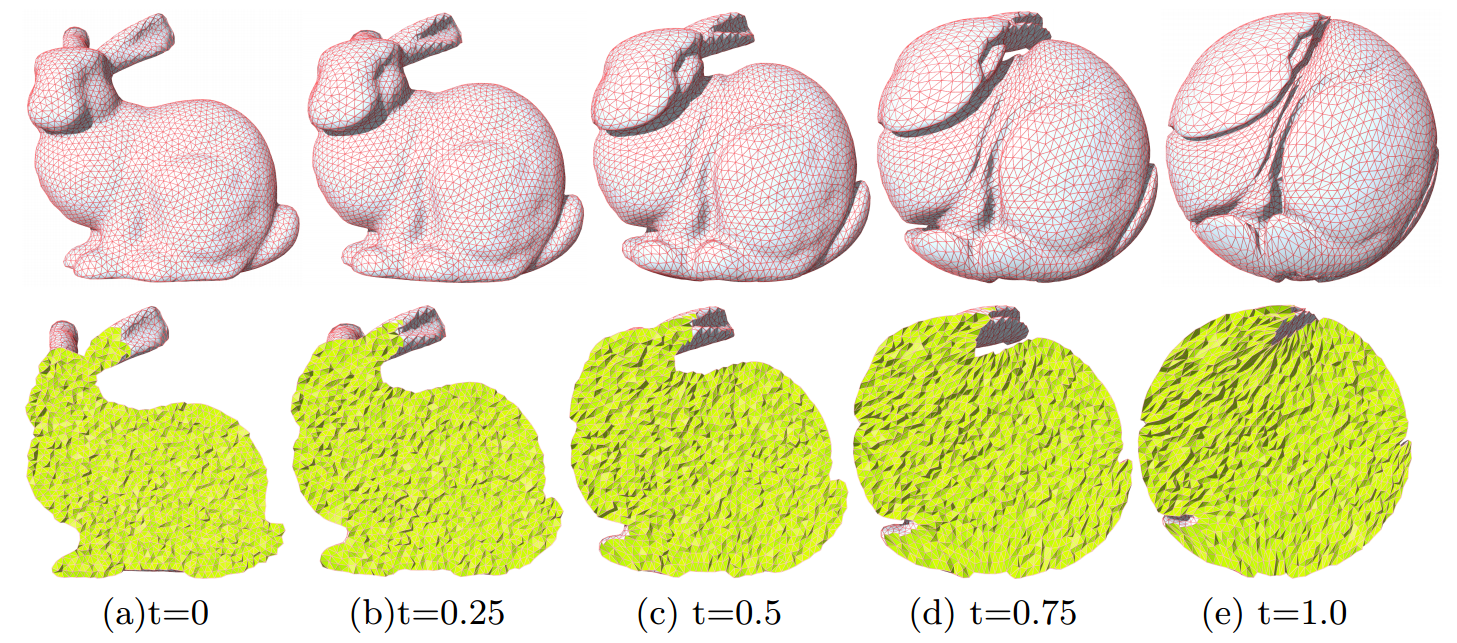
\includegraphics[width= 0.9 \textwidth]{figs/bruno.png}

}
\caption{The volume morphing of Bunny(side view)using Bruno Levy method at typical time}
\label{fig:bruno_morph}
\end{figure}
\end{frame}


\begin{frame}{Volume Preserving Parameterization}
\begin{figure}
\centering
\makebox[\textwidth]{

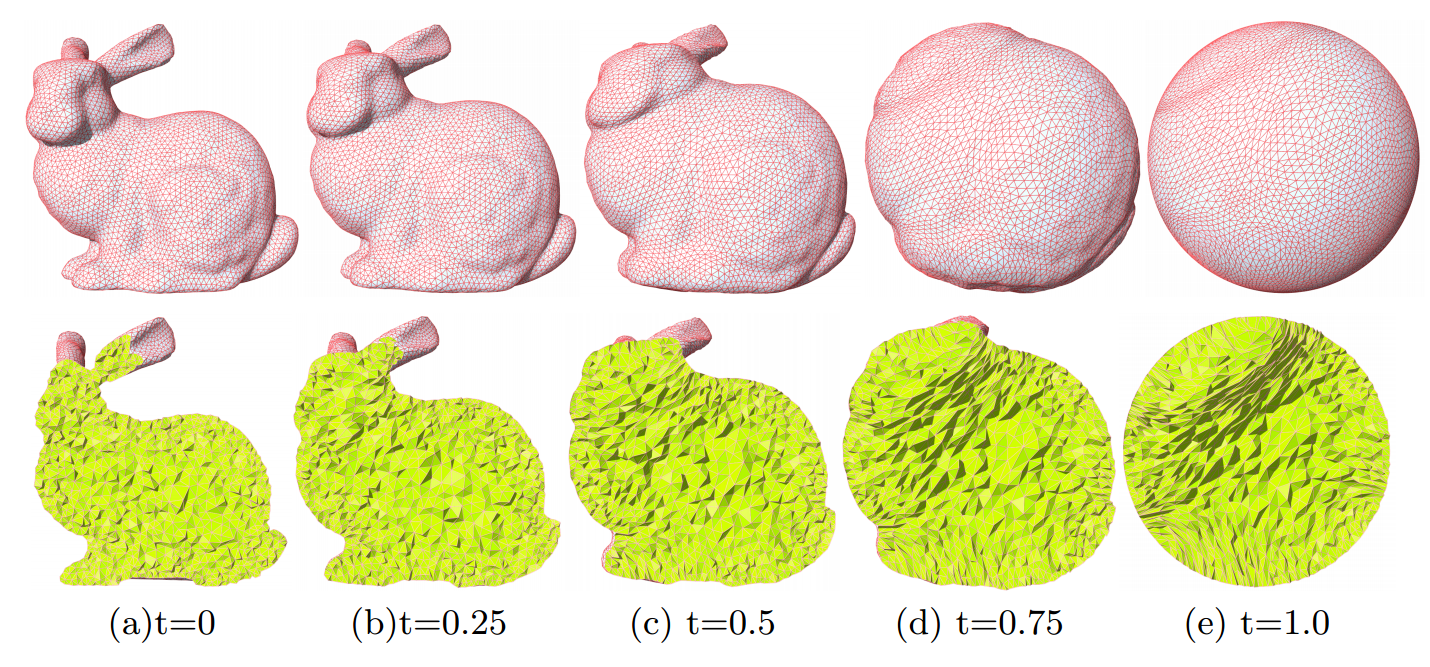
\includegraphics[width= 0.9 \textwidth]{figs/gu.png}

}
\caption{The volume morphing of Bunny(side view)using OMT at typical time}
\label{fig:gu_morph}
\end{figure}
\end{frame}

\section{Conclusion}



\begin{frame}{Conclusion}
In this presentation, I introduce the history of Optimal Mass Transport(OMT) and our present research approach and result of OMT. 

\begin{enumerate}

\item Brenier's polar factorization\cite{brenier1991polar} and Yau-Luo-Gu's\cite{gu2013variational} variational principle method establish the bridge to link  $ Minkowski-Alexandrov $ problem and $ Monge-Kantorovich $ problem.

\item Introduce the Wasserstein distance to describe the similarity of two Riemannian surfaces. 

\item  OMT and Wasserstein distance's applications in Shape Analysis, Visualization and Volume-Preserving morphing or Volume Parameterization.

\end{enumerate}


\end{frame}

\section{Future Works}
\begin{frame}{Future Works}
In future, there are three directions need more effort.

\begin{enumerate}

\item  High dimension OMT algorithm
\item  OMT Map in $3D$ human face tracking
\item  Volume parametrization
\end{enumerate}

\end{frame}



\bibliographystyle{unsrt}
\bibliography{egbib}

\end{document}


